\chapter{Wireless standards and protocols}
\label{wireless-standards-and-protocols}

\textbf{Wireless sucks:} vengono persi pacchetti, servono
regolamentazioni delle frequenze, canale di comunicazione non limitabile
e condiviso, scarsa sicurezza, trasmissione lenta e variabile, ecc.

Però fa comodo perché è veloce da installare e richiede poca
infrastruttura.

L'obiettivo finale è quello di andare a pila di reti wireless che sia in
grado di connettere aree geografiche molto ampie, garantendo allo stesso
tempo una buona velocità di trasmissione.

\subsection{Tecnologie correnti}\label{tecnologie-correnti}

\begin{itemize}
\item
  \begin{quote}
  \textbf{Mobile Cellular Systems:} utilizzata per far comunicare i
  telefoni ed effettuare principalmente traffico voce. Gli access point
  coprono dai 100 metri ai 10km ma garantiscono una velocità di
  trasmissione contenuta.
  \end{quote}
\item
  \begin{quote}
  \textbf{WLAN}: estensione wireless della rete ethernet con copertura
  più limitata, dai 10 ai 100 metri. Aumenta però la velocità di
  trasmissione.
  \end{quote}
\item
  \begin{quote}
  \textbf{Short-range}: connessione diretta tra dispositivi, ottimizzata
  per contenere i consumi.
  \end{quote}
\item
  \begin{quote}
  \textbf{Satellite systems}: connessione satellitare in grado di
  coprire tutto il mondo, utilizzata per trasmissioni audio/video.
  \end{quote}
\end{itemize}

\subsection{Enti per le
standardizzazioni}\label{enti-per-le-standardizzazioni}

\begin{itemize}
\item
  \begin{quote}
  \textbf{3GPP}: GSM, UMTS, LTE
  \end{quote}
\item
  \begin{quote}
  \textbf{IEEE:} 802.x (LAN, PAN; WiMAX)
  \end{quote}
\item
  \begin{quote}
  \textbf{IETF (Internet Engineering Task Force)}: Mobile IP,
  TCP...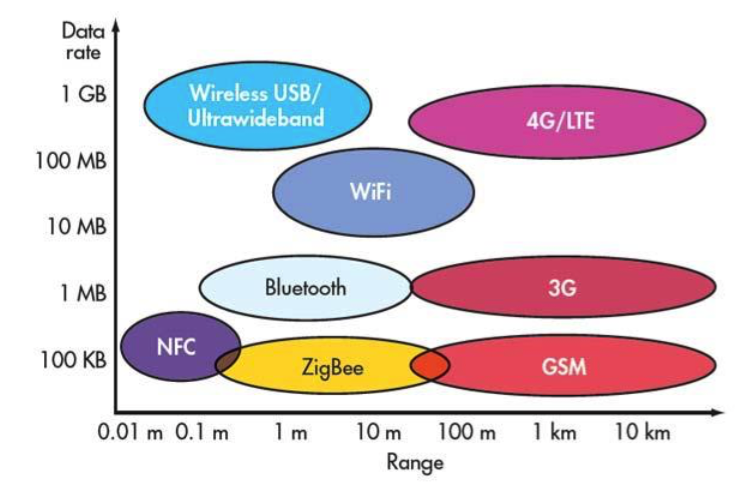
\includegraphics[width=5.00521in,height=3.05208in]{image10.png}
  \end{quote}
\end{itemize}

\subsection{802.11 Wireless Local Area
Network}\label{wireless-local-area-network}

802.X è una famiglia di standard per le reti locali e metropolitane, in
particolare 802.11 definisce il \textbf{MAC (Medium Access Control)} e
il \textbf{PHY (Physical layer)} per le reti wireless.

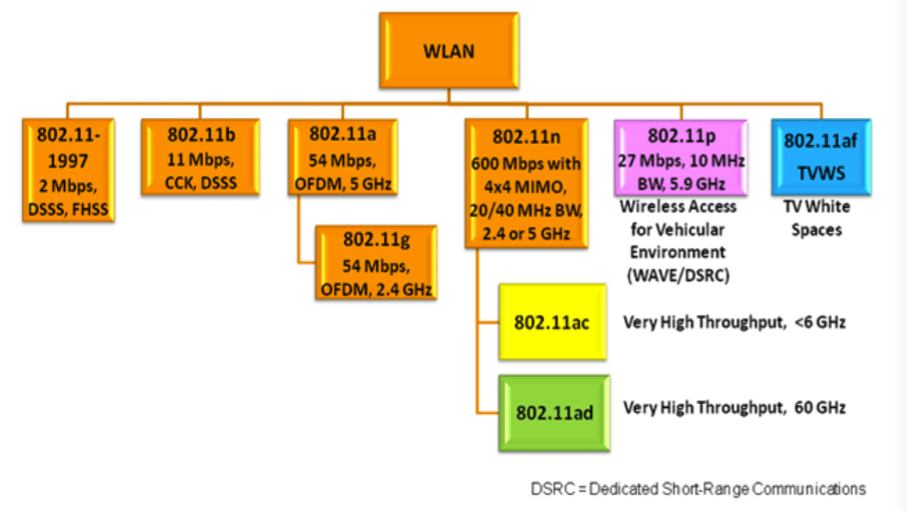
\includegraphics[width=6.26772in,height=3.52778in]{image8.png}

L'obiettivo prefissato per 802.11 è quello di permettere di connettersi
a reti wireless secondo uno standard unico per tutto il mondo, che non
richiede licenze, facile da usare e che consuma poco. Anche la sicurezza
e la privacy devono essere garantite.

Viene quindi definita una pila di protocolli che specifica come avviene
la comunicazione tra i vari
dispositivi.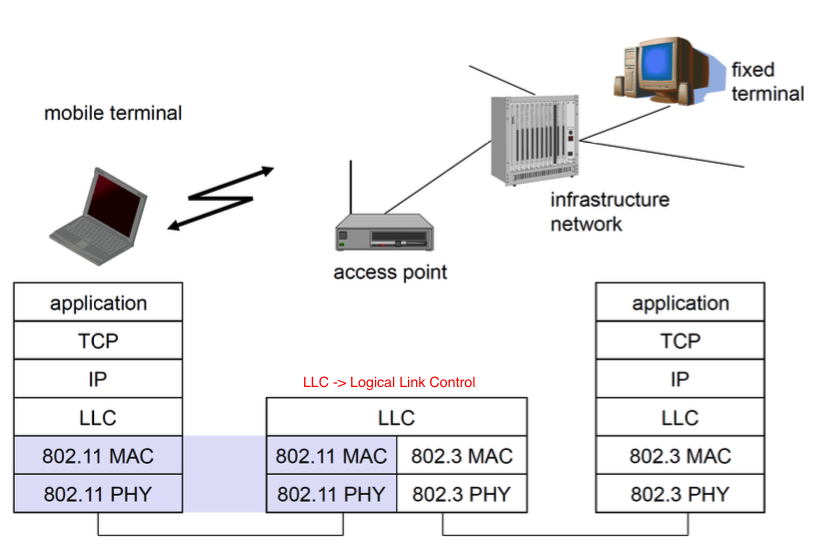
\includegraphics[width=5.29395in,height=3.53844in]{image6a.png}

L'utilizzo tipico prevede un dispositivo mobile che si connette ad un
access point mediante 802.11, l'accesso point è inoltre connesso
all'infrastruttura cablata tramite 802.3, il che permette al dispositivo
mobile di comunicare con tutti i dispositivi connessi alla rete cablata.

Più nel dettaglio, gli strati del MAC e PHY layer sono divisi in vari
componenti:

\begin{itemize}
\item
  \begin{quote}
  \textbf{MAC:} si occupa del meccanismo di accesso al canale, della
  frammentazione dei pacchetti e dell'encryption dei dati.
  \end{quote}
\item
  \begin{quote}
  \textbf{MAC Management}: contiene la logica di sincronizzazione e
  autenticazione
  \end{quote}
\item
  \begin{quote}
  \textbf{PLCP Physical Layer Convergence Protocol:} controlla il canale
  di comunicazione
  \end{quote}
\item
  \begin{quote}
  \textbf{PMD Physical Medium Dependent}: si occupa della codifica e
  modulazione del segnale.
  \end{quote}
\item
  \begin{quote}
  \textbf{Station Management}: si occupa di tutte le funzionalità legate
  alla gestione della stazione di trasmissione.
  \end{quote}
\end{itemize}

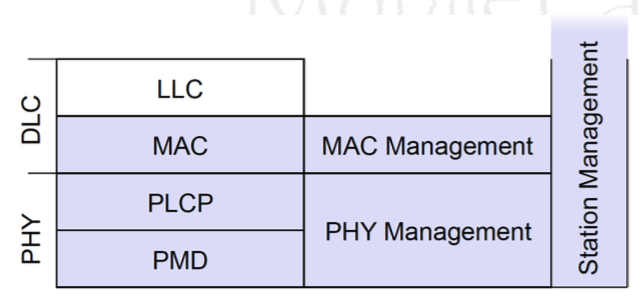
\includegraphics[width=3.98438in,height=1.83334in]{image12.png}

L'accesso al canale viene fatto con \textbf{CSMA/CA: Carrier Sense
Multiple Access with Collision Avoidance}, ovvero prima di effettuare
una trasmissione viene controllato il canale e viene effettuata una
trasmissione solo se questo è libero. Questo perché non è possibile
effettuare Collision detection.

Ci sono varie versioni dello standard 802.11, ognuna delle quali
definisce particolari velocità di trasmissioni, frequenze e
caratteristiche del dispositivo di trasmissione/modulazione del segnale.

Per gestire la convivenza di più reti wireless è stato predisposto un
meccanismo di canali che utilizzano frequenze di trasmissioni diverse.

\subsubsection{Infrastruttura Vs Ad-Hoc network Vs Wi-Fi
Direct}\label{infrastruttura-vs-ad-hoc-network-vs-wi-fi-direct}

\paragraph{Infrastruttura }\label{infrastruttura}

Tipicamente 802.11 viene utilizzato in modalità \textbf{Infrastruttura},
ovvero ci sono degli access point che collegano una rete wireless ad una
rete cablata, in modo che i dispositivi mobile possono usufruire degli
stessi servizi.

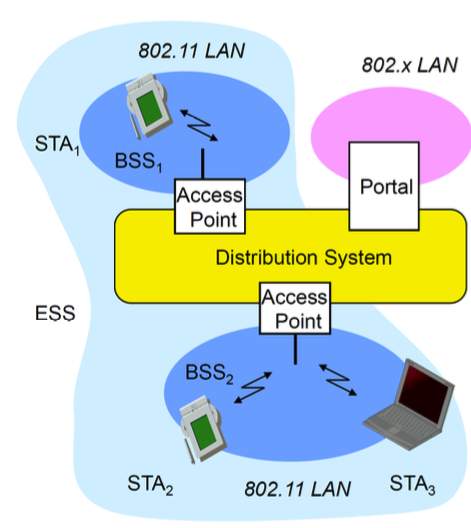
\includegraphics[width=2.88308in,height=3.23438in]{image7.png}

In questo caso si hanno delle \textbf{Station (STA)} che sono dei
terminali con accesso alla rete wireless e che sono in grado di
comunicare con l'access point. Vengono poi identificati vari \textbf{BSS
(Basic Service Set)} che definiscono un gruppo di stazioni che
comunicano sulla stessa frequenza radio. Un \textbf{Access Point} è una
particolare stazione che è connessa sia alla rete wireless che al
sistema di distribuzione dell'infrastruttura (tipicamente la rete
cablata). Un \textbf{Portal} è un ponte che permette la comunicazione
tra due reti diverse (da notare che non è tra AP ad AP), come tra la
rete wireless e quella wired. Il \textbf{Distribution System} è un
interconnessione di reti eterogenee definite da vari \textbf{BSS} che
formano un'unica rete logica che prende il nome di \textbf{Extended
Service Set (ESS)}.

Il set-up della rete wireless viene gestito da un amministratore, il
quale stabilisce i canali di trasmissione dei vari access point, stando
attendo a limitare le interferenze. I vari host si connetteranno poi a
uno degli access point secondo il seguente procedimento:

\begin{enumerate}
\def\labelenumi{\arabic{enumi}.}
\item
  \begin{quote}
  Ascoltano il canale per cercare dei \textbf{beacon frame} che
  descrivono l'access point (nome \textbf{SSID} e MAC address).
  \end{quote}
\item
  \begin{quote}
  Selezionano l'access point a cui associarsi.
  \end{quote}
\item
  \begin{quote}
  Effettuano l'autenticazione (opzionale)
  \end{quote}
\item
  \begin{quote}
  Ottengono un IP, tipicamente assegnato in DHCP, valido per la
  sotto-rete definita dall'access point.
  \end{quote}
\end{enumerate}

Una volta associato o connesso, l'host comunicherà con tutti gli altri
host collegati in rete mediante l'access point (no connesione diretta).

\paragraph{Ad Hoc}\label{ad-hoc}

Nella modalità \textbf{Ad-Hoc} la comunicazione è invece limitata
all'interno di un singolo \textbf{BSS}, che in questo caso prende il
nome di \textbf{Independent Basic Service Set}, in quanto non è
collegato con un sistema di distribuzione.

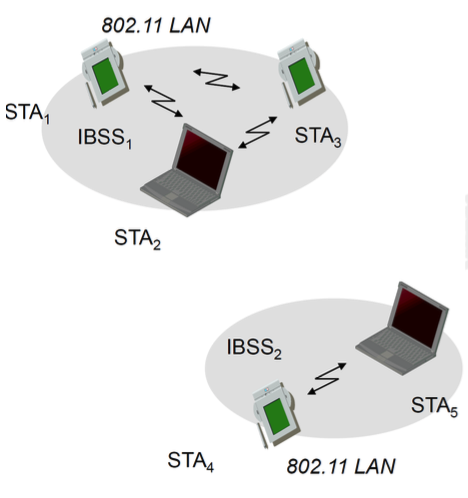
\includegraphics[width=3.11785in,height=3.31771in]{image11.png}

In questo caso il meccanismo di creazione della rete e associazione è
diverso. In primo luogo è necessario un dispositivo che sia in grado di
avviare un \textbf{IBSS} che inizia a trasmettere un beacon con SSID,
BSSID e TSF (timer value). Gli altri dispositivi si connettono alla rete
così creata e a turno si prendono l'onere di trasmettere il beacon
identificativo. In questo caso non ci sono obblighi legati alla
sicurezza/crittografia/autenticazione.

\paragraph{WiFi-Direct o P2P}\label{wifi-direct-o-p2p}

Application layer che permette a due dispositivi di connettersi tra loro
senza passare per l'infrastruttura. Questo avviene perché un device
agisce come soft access point (AP) o \textbf{group-owner} (\textbf{GO}),
mentre gli altri si connettono come se fossero delle normali stazioni,
con la differenza che i ruoli all'interno del gruppo possono cambiare
nel tempo a seguito di una negoziazione. In ogni caso l'ownership del
gruppo non può essere trasferita.

La scoperta di un nuovo gruppo avviene inviando un particolare messaggio
\emph{Probe} \emph{P2P Information elements} al quale un altro
dispositivo che supporta il P2P o un GO possono rispondere. Il messaggio
inviato contiene la descrizione del device che l'ha inviato.

La differenza principale con le Reti Mobile Ad-Hoc (\textbf{MANET}) è
che con WiFi-Direct i dispositivi negoziano tra di loro per decidere
quale dispositivo farà da access-point e quindi si avrà una
\emph{single-hop} \emph{communication} verso l'unico access point,
mentre in una MANET ogni device è in grado di indirizzare i propri
messaggi all'interno dell'IBSS.

I vantaggi di MANET rispetto a WiFi-Direct riguardano principalmente la
robustezza/efficienza della rete, ma sono più difficili da configurare,
mentre WiFi-Direct è in grado di configurarsi automaticamente e prevede
in automatico la crittografia dei messaggi, ma il set-up automatico
richiede un lungo scambio di messaggi e la rete creata non è molto
flessibile.

La creazione di un gruppo Wi-Fi Direct avviene prima con lo scambio di
messaggi \emph{Probe} per capire quali dispositivi sono interessati alla
creazione del gruppo, dopodiché viene effettuata la negoziazione del
\textbf{GO}. Una volta stabilito il GO, viene effettuata la fase di
\textbf{WPS (WiFi Proteced Set Up)} ed infine vengono stabiliti gli IP
locali mediante DHCP. Ovviamente se c'è un gruppo già formato,
identificabile dal SSID della rete che deve iniziare con
DIRECT-randomNumber non vengono fatte le fasi di
\emph{Probe}-\emph{Negotiation,} ma si passa subito al WPS.

\subsection{802.15 Personal Area Network}\label{personal-area-network}

L'obiettivo di questo standard è di definire una rete wireless a corto
raggio e con consumi ridotti.
